\section{Meilenstein 2: 24.05.2019 - 22.05.2019}
Der zweite Meilenstein hat das Ziel den Main Showcase abzubilden und so gleichzeitig den technischen Durchstich durch alle Komponenten unseres Systems aufzuzeigen.
Das bedeutet, dass die Sensorknoten in der Lage sind, Daten zu messen und an die IoT-Plattform zu senden.
In der IoT-Plattform werden diese Daten aufgenommen und in einer Datenbank abgespeichert.
Um mit den gespeicherten Daten weiterarbeiten zu können, müssen die Daten über einen Service bei der IoT-Plattform abgefragt werden können.
Diese Daten werden dann von dem Routing-Service genutzt, indem sie in der Berechnung einer Route als Gewichtungsfaktor berücksichtigt werden.
So kann letztendlich die Navigationsapplikation über einen Schnittstelle zum Routing-Algorithmus einen Start- und Endpunkt übergeben, aus welchen eine Route erstellt wird, die man über eine weitere Schnittstelle dem Navigationsnutzer bereitstellt.

Das übergeordnete Ziel des Meilensteins ist es also nicht nur, den technischen Durchstich zu erwirken, sondern auch ein Zusammenspiel aller Komponenten untereinander zu schaffen.
Um dies zu ermöglichen ist es notwendig, dass unter den unterschiedlichen Komponenten beziehungsweise Gruppen Schnittstellen implementiert werden, die zuvor in der Architektur festgelegt worden sind.
Um dieses Ziel zu erreichen, ist ein hoher Abstimmungsaufwand erforderlich sowie das Durchführen von Integrationstests, um sicherzustellen, dass die Schnittstellen zwischen den einzelnen Komponenten funktionsfähig sind.


Zusammenfassend zum zweiten Meilenstein lässt sich festhalten, dass nicht alle geplanten Ziele erreicht werden konnten.
Ein Gesamtbild der Ergebnisse zeigt sich in \Fig{bigpicture1}.
In dieser Abbildung werden zu jedem der vier Teilbereiche die vorher gesetzten Ziele aufgelistet.
Zudem wird farblich gekennzeichnet, ob die Ziele vollständig (grün), zum Teil(gelb) oder gar nicht (rot) erreicht wurden.
Dabei muss berücksichtigt werden, dass es sich bei den Zielen nur um die gesetzten Ziele im Meilenstein handelt und nicht um die Gesamtziele im Projekt.

\begin{figure}[!htb]
	\centering
	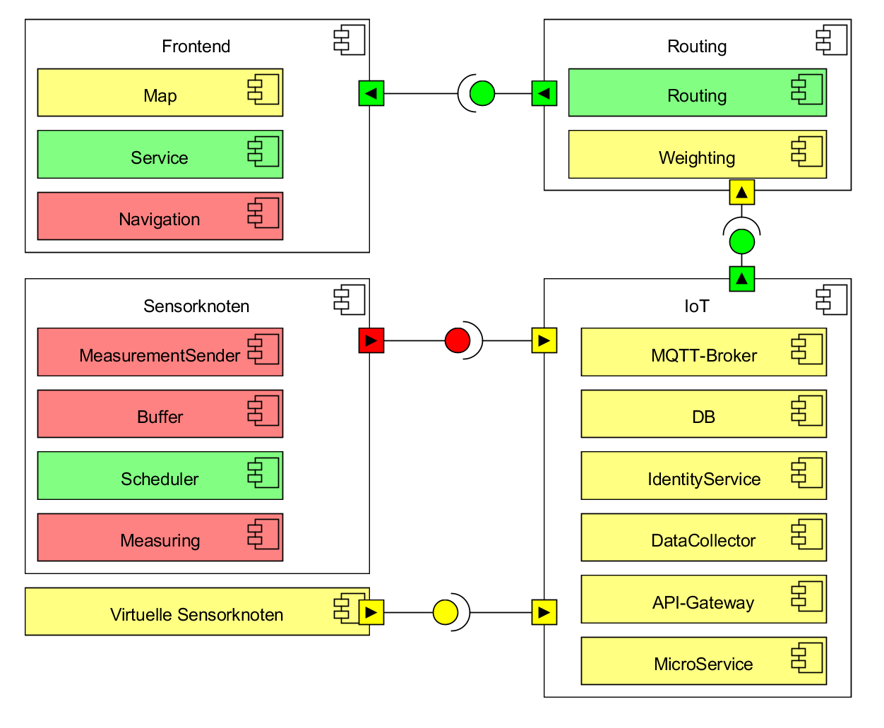
\includegraphics[width=\textwidth]{./ressourcen/bigpicture1.png}
	\caption{Big Picture des ersten Meilensteins}
	\label{fig:bigpicture1}
\end{figure}

In dem Gesamtbild zu den Meilensteinzielen zeigt sich deutlich, dass nicht alle Ziele vollständig erreicht werden konnten.
Unter anderem konnten Themen im Bereich Sensorknoten und Frontend gar nicht erst angegangen werden.
Dies hat verschiedene Gründe: Zum einen ist dieser Meilenstein der erste, bei dem die Projektgruppe mit tatsächlichen Anforderungen aus Sicht eines Nutzers gearbeitet hat.
Das Ergebnis dessen ist, dass viele Aufwände noch falsch eingeschätzt wurden.
Am deutlichsten zeigt sich dies bei der Entwicklung der Firmware für die Sensorknoten und den zu entwickelnden Komponenten der IoT"=Plattform.
So konnte insgesamt kein vollständiger technischer Durchstich des Systems aufgezeigt werden, da zum Beispiel der MeasurementSender der Sensorknoten Firmware noch nicht funktionsfähig war und zudem auch noch keine Schnittstelle zwischen der IoT"=Plattform und dem Sensorknoten zur Verfügung stand.
Dem gegenüber stehen jedoch das nahezu vollständige Erreichen der Ziele in anderen Komponenten wie Routing sowie die Schnittstellen zwischen Routing, IoT und Frontend.
Bei der Bewertung muss jedoch berücksichtigt werden, dass sowohl die Aufwände als auch Einarbeitungszeiten in nahezu allen Gruppen falsch eingeschätzt wurden.
Der Meilenstein hat deutlich aufgezeigt, dass die Gruppeneinteilung sowie die Schätzung der Aufwände an den Jira"=Tickets noch weiter optimiert werden muss.
Der Grund für das nicht"=erreichen der Ziele des zweiten Meilensteins ist nicht darin begründet, dass zu wenig Aufwand von den Mitgliedern der Projektgruppe betrieben wurden, sondern lediglich die Ziele nach einem so kurzen Zeitraum signifikant zu hoch gesteckt wurden.